\documentclass{beamer}
    \usefonttheme{serif}
\usepackage{fontspec}
    \setmainfont{MLMRoman10}
    \setsansfont{MLMSans10}
    \setmonofont{MLMMono10}
\usepackage{subcaption}
\usepackage{verbatim}
\usepackage{tikz}
    \usetikzlibrary{positioning, arrows.meta}

\title{Ain't Detokenization A Kick In The Head?}
\subtitle{An Interventional Study of Specialized Attention Heads \\ in Early Word Reconstruction}
\author{Gustaf Gren}
\date{}

\begin{document}

\begin{frame}
  \titlepage
\end{frame}

\begin{frame}{Detokenization in LLMs}

\textbf{20 pages in one sentence}: \\
Are there attention heads crucial for \textit{detokenization}, an early stage of inference in LLMs responsible for combining tokens to more coherent units?

\begin{figure}[ht]
\centering

\begin{subfigure}{0.45\textwidth}
\centering
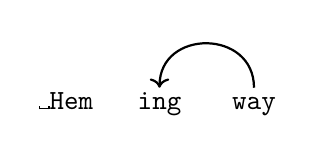
\begin{tikzpicture}[baseline, every node/.style={text height=1ex, text depth=.25ex}, node distance=1.2cm]
\node (1) {\texttt{␣Hem}};
\node (2) [right of=1] {\texttt{ing}};
\node (3) [right of=2] {\texttt{way}};
\draw[->, thick] (3.north) to[out=90,in=90,looseness=1.6] (2.north);
\end{tikzpicture}
\caption{in-boundary}
\end{subfigure}
\hfill
\begin{subfigure}{0.45\textwidth}
\centering
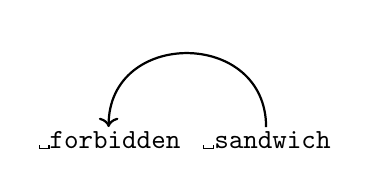
\begin{tikzpicture}[baseline, every node/.style={text height=1ex, text depth=.25ex}, node distance=2cm]
\node (1) {\texttt{␣forbidden}};
\node (2) [right of=1] {\texttt{␣sandwich}};
\draw[->, thick] (2.north) to[out=90,in=90,looseness=1.6] (1.north);
\end{tikzpicture}
\caption{out-boundary}
\end{subfigure}
\end{figure}

\end{frame}

\begin{frame}{Testing}
\begin{exampleblock}{Example input sequence}
\small{
\texttt{['Sal', '␣Paradiso', '␣lives', '␣in', '␣Pat', \textbf{\textcolor{red}{'erson'}}]}
}
\end{exampleblock}

\bigskip
\begin{block}{Activation Patching}
\texttt{"Repeat the following word: \textcolor{red}{X}, \textcolor{red}{X}, \textcolor{red}{X},"}
\medskip

Patch each layer's hidden state to \texttt{X} to reconstruct the full word (e.g., \texttt{'erson'} $\rightarrow$ 'Paterson') under different ablation (setting attention head output to 0) levels (1/3/5\%), random ablation control, and normal forward pass.
\end{block}

\bigskip
We test using Toksuite (models which are similar except tokenizer), and Qwen2.5 under different parameter sizes (0.5B-7B).
\end{frame}


\begin{frame}{Takeaways}
\begin{itemize}
\item Specific attention heads seem to drive multi-token word representations.
\item Zeroing these heads \textbf{hurts retrieval} (random not too bad)
\item Results suggest:
    \begin{enumerate}
        \item Larger models show \textit{specialized attention}.
        \item The tokenizer impacts learning efficiency for representations.
    \end{enumerate}
\end{itemize}
\end{frame}

\end{document}
